% File: slides/01_introduction.tex

% --- Slide 1: Tên luận văn ---
\begin{frame}
    \centering
    {\LARGE \TENLUANVAN \par}
    \vspace{0.5cm}
    {\large \textit{\THESISNAME} \par}
\end{frame}

% --- Slide 2: Thông tin tác giả ---
\begin{frame}
    \centering
    {\Large Tác giả: \TENTACGIA \par}
    {\Large Người hướng dẫn: \TENNGUOIHUONGDAN \par}
    \vspace{0.5cm}
    {\small Khoa: \KHOA \par}
    {\small Trường: \TRUONG \par}
    \vfill
    {\footnotesize \today}
\end{frame}

% --- Slide 3: Té ngã – Vấn đề toàn cầu ---
\begin{frame}
    \frametitle{Té ngã – Vấn đề toàn cầu}
    \begin{columns}[T]
        \begin{column}{0.48\textwidth}
            \begin{itemize}
                \item Nguyên nhân chính gây chấn thương nghiêm trọng \& tử vong.
                \item WHO: $\sim 646{,}000$ ca/năm; $>80\%$ ở nước thu nhập trung bình/thấp.
                \item Người cao tuổi ($>65$ tuổi): 30\% té ngã/năm; $>85$ tuổi: 50\%.
            \end{itemize}
        \end{column}
        \begin{column}{0.48\textwidth}
            \begin{figure}
                \centering
                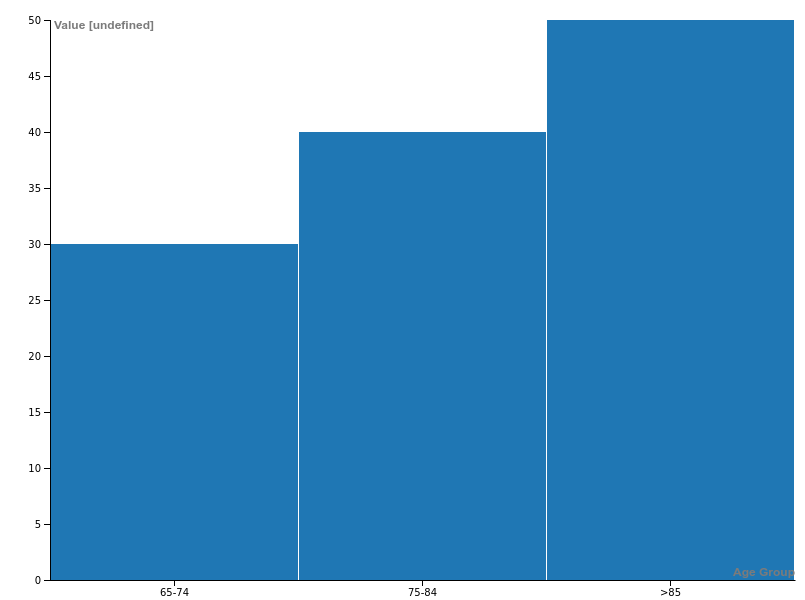
\includegraphics[width=\textwidth]{images/fall_status_who.png}
                \caption{Tỷ lệ té ngã theo nhóm tuổi (WHO)}
            \end{figure}
        \end{column}
    \end{columns}
\end{frame}

% --- Slide 4: Hệ thống phát hiện té ngã ---
\begin{frame}
    \frametitle{Hệ thống phát hiện té ngã}
    \begin{itemize}
        \item Giám sát chuyển động bằng cảm biến: IMU, gyroscope, cảm biến áp suất.
        \item Phân tích hình ảnh thời gian thực từ camera cố định.
        \item Cảnh báo nhanh qua GPS, gửi thông tin đến người thân và nhân viên y tế.
        \item Trọng tâm: xây dựng \& tối ưu hệ thống phát hiện và cảnh báo té ngã.
    \end{itemize}
\end{frame}

% --- Slide 5: Tình hình nghiên cứu ---
\begin{frame}
    \frametitle{Tình hình nghiên cứu trong và ngoài nước}
    \begin{columns}[T]
        \begin{column}{0.5\textwidth}
            \textbf{Phương pháp chính:}
            \begin{itemize}
                \item Vision-based: camera + phân tích tư thế
                \item Wearable sensor-based: IMU, accelerometer, gyroscope
                \item Multi-modal: kết hợp nhiều nguồn dữ liệu
            \end{itemize}
        \end{column}
        \begin{column}{0.5\textwidth}
            \textbf{Nghiên cứu quốc tế:}
            \begin{itemize}
                \item Vision-based: OpenPose, MediaPipe, MoveNet; F1 $\sim 91\%$
                \item Kết hợp YOLO + Pose Estimation: mAP 92--98\%, edge devices
                \item Wearable \& Multi-modal: LSTM + IMU, accuracy 93--95\%, giảm ER visits $\sim 80\%$
            \end{itemize}
        \end{column}
    \end{columns}
\end{frame}

% --- Slide 6: Nghiên cứu trong nước \& cơ hội ---
\begin{frame}
    \frametitle{Nghiên cứu trong nước \& cơ hội}
    \begin{columns}[T]
        \begin{column}{0.5\textwidth}
            \textbf{Trong nước:}
            \begin{itemize}
                \item Proof-of-concept: Arduino, ESP32, IMU; accuracy 75--85\%
                \item Cảnh báo SMS/app di động cơ bản
                \item Tập trung đánh giá nguy cơ té ngã, thang Morse, dự báo
            \end{itemize}
        \end{column}
        \begin{column}{0.5\textwidth}
            \textbf{Cơ hội:}
            \begin{itemize}
                \item Áp dụng AI + IoT: nâng cao accuracy, giảm false alarm
                \item Adaptive sensor fusion, edge computing
                \item Nghiên cứu dữ liệu lớn, cải thiện triển khai thực tế
            \end{itemize}
        \end{column}
    \end{columns}
\end{frame}

% --- Slide 7: Mục tiêu Luận Văn ---
\begin{frame}
    \frametitle{Mục tiêu Luận Văn}
    \begin{columns}[T]
        \begin{column}{0.48\textwidth}
            \begin{itemize}
                \item Giám sát \& cảnh báo té ngã thông minh cho người cao tuổi/bệnh nhân
                \item Phát hiện real-time, xử lý dữ liệu cảm biến \& hình ảnh
                \item Kiến trúc phân lớp, ổn định, chi phí thấp, dễ mở rộng
            \end{itemize}
        \end{column}
        \begin{column}{0.48\textwidth}
            \begin{figure}
                \centering
                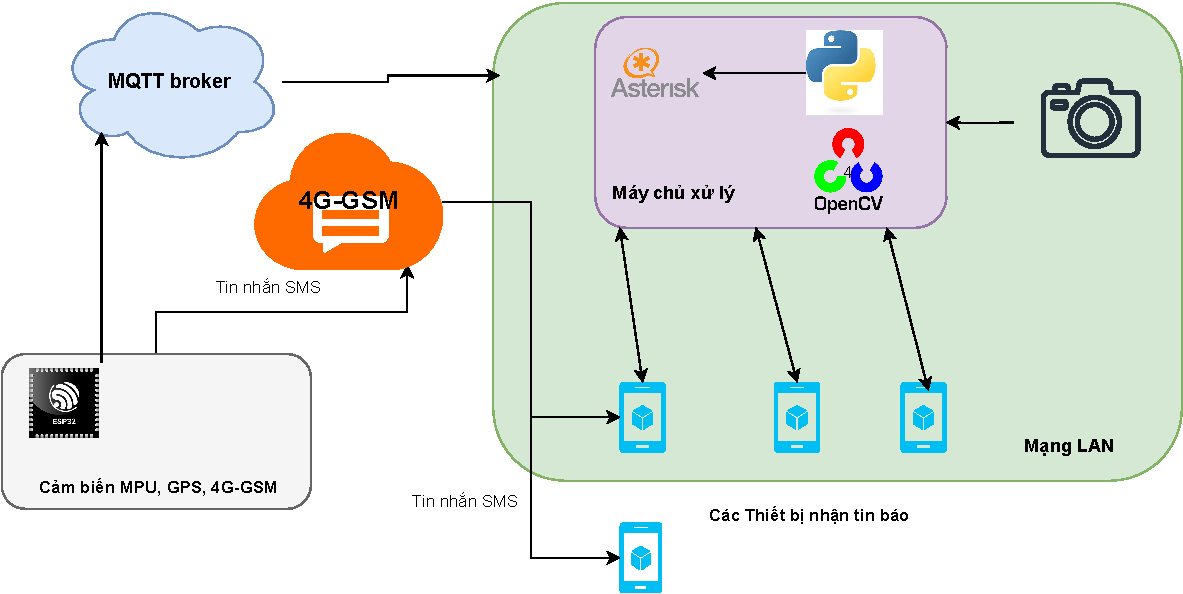
\includegraphics[width=\textwidth]{images/resuilt_structure_diagram.pdf}
                \caption{Sơ đồ hệ thống tổng thể}
            \end{figure}
        \end{column}
    \end{columns}
\end{frame}

% --- Slide 8: Hệ thống phân tích hình ảnh ---
\begin{frame}
    \frametitle{Hệ thống phân tích hình ảnh}
    \begin{columns}[T]
        \begin{column}{0.48\textwidth}
            \begin{itemize}
                \item MediaPipe, OpenCV, YOLO: trích xuất keypoints, phân tích tư thế
                \item Pipeline: góc nghiêng $\rightarrow$ vận tốc $\rightarrow$ tỉ lệ khung xương $\rightarrow$ nhận diện té ngã
                \item Huấn luyện ML (SVM, Decision Tree) trên tập dữ liệu tư thế
            \end{itemize}
        \end{column}
        \begin{column}{0.48\textwidth}
            \begin{figure}
                \centering
                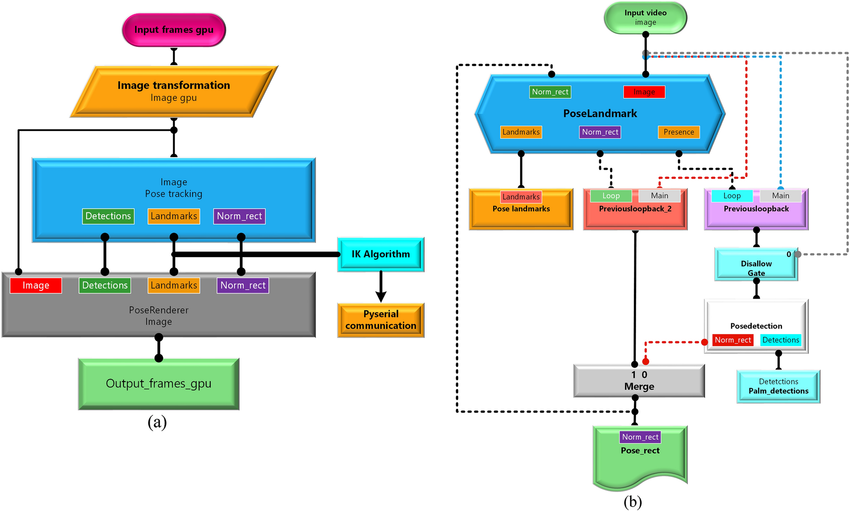
\includegraphics[width=\textwidth]{images/media_pose_pipeline.png}
                \caption{Pipeline MediaPipe + YOLO}
            \end{figure}
        \end{column}
    \end{columns}
\end{frame}

% --- Slide 9: Hệ thống nhúng ESP32 ---
\begin{frame}
    \frametitle{Hệ thống nhúng ESP32}
    \begin{columns}[T]
        \begin{column}{0.48\textwidth}
            \begin{itemize}
                \item ESP32 + MPU6050 + GPS EC800K
                \item Phát hiện té ngã theo ngưỡng động học
                \item Internet: MQTT ; SMS 
                \item Thiết bị độc lập, tiết kiệm năng lượng, mở rộng được
            \end{itemize}
        \end{column}
        \begin{column}{0.48\textwidth}
            \begin{figure}
                \centering
                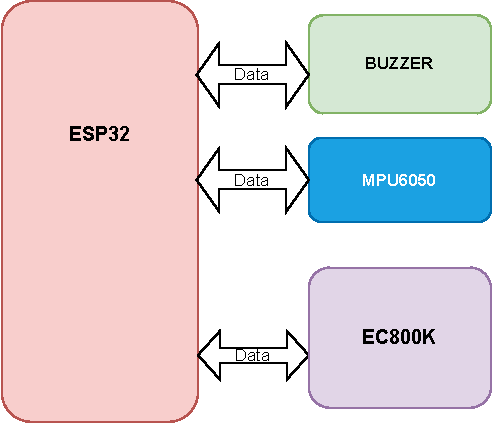
\includegraphics[width=\textwidth]{images/module1_block_diagram-crop.pdf}
                \caption{Sơ đồ nhúng ESP32 \& truyền thông}
            \end{figure}
        \end{column}
    \end{columns}
\end{frame}

% --- Slide 10: Hiệu năng \& Giới hạn ---
\begin{frame}
    \frametitle{Hiệu năng \& Giới hạn}
    \begin{columns}[T]
        \begin{column}{0.48\textwidth}
            \textbf{Mục tiêu:}
            \begin{itemize}
                \item Tổng độ trễ $<$5 giây
                \item Accuracy $>$90\%, false alarm $<$8\%
                \item Uptime SIP/MQTT $>$99\%
                \item Hỗ trợ nhiều node cảm biến
            \end{itemize}
        \end{column}
        \begin{column}{0.48\textwidth}
            \textbf{Giới hạn:}
            \begin{itemize}
                \item Chỉ trong nhà, ánh sáng đủ, mạng ổn định
                \item ESP32 prototype chưa học sâu toàn phần
                \item Không phát triển app di động/web phức tạp
                \item Sử dụng Linux \& MQTT broker sẵn có
            \end{itemize}
        \end{column}
    \end{columns}
\end{frame}

% --- Slide 11: Phạm vi nghiên cứu ---
\begin{frame}
    \frametitle{Phạm vi nghiên cứu}
    \begin{itemize}
        \item \textbf{Kỹ thuật \& công nghệ:} ESP32, MPU6050, GPS, MediaPipe, OpenCV, MQTT, SIP/Asterisk
        \item \textbf{Chức năng:} Phát hiện té ngã real-time, cảnh báo đa kênh
        \item \textbf{Dữ liệu \& môi trường:} Camera cố định, indoor, ánh sáng đủ, kết nối ổn định
        \item \textbf{Giới hạn:} Không tối ưu môi trường thiếu sáng, ngoài trời; không phát triển giao diện phức tạp
    \end{itemize}
\end{frame}

